\begin{figure}[ht]
    \centering
    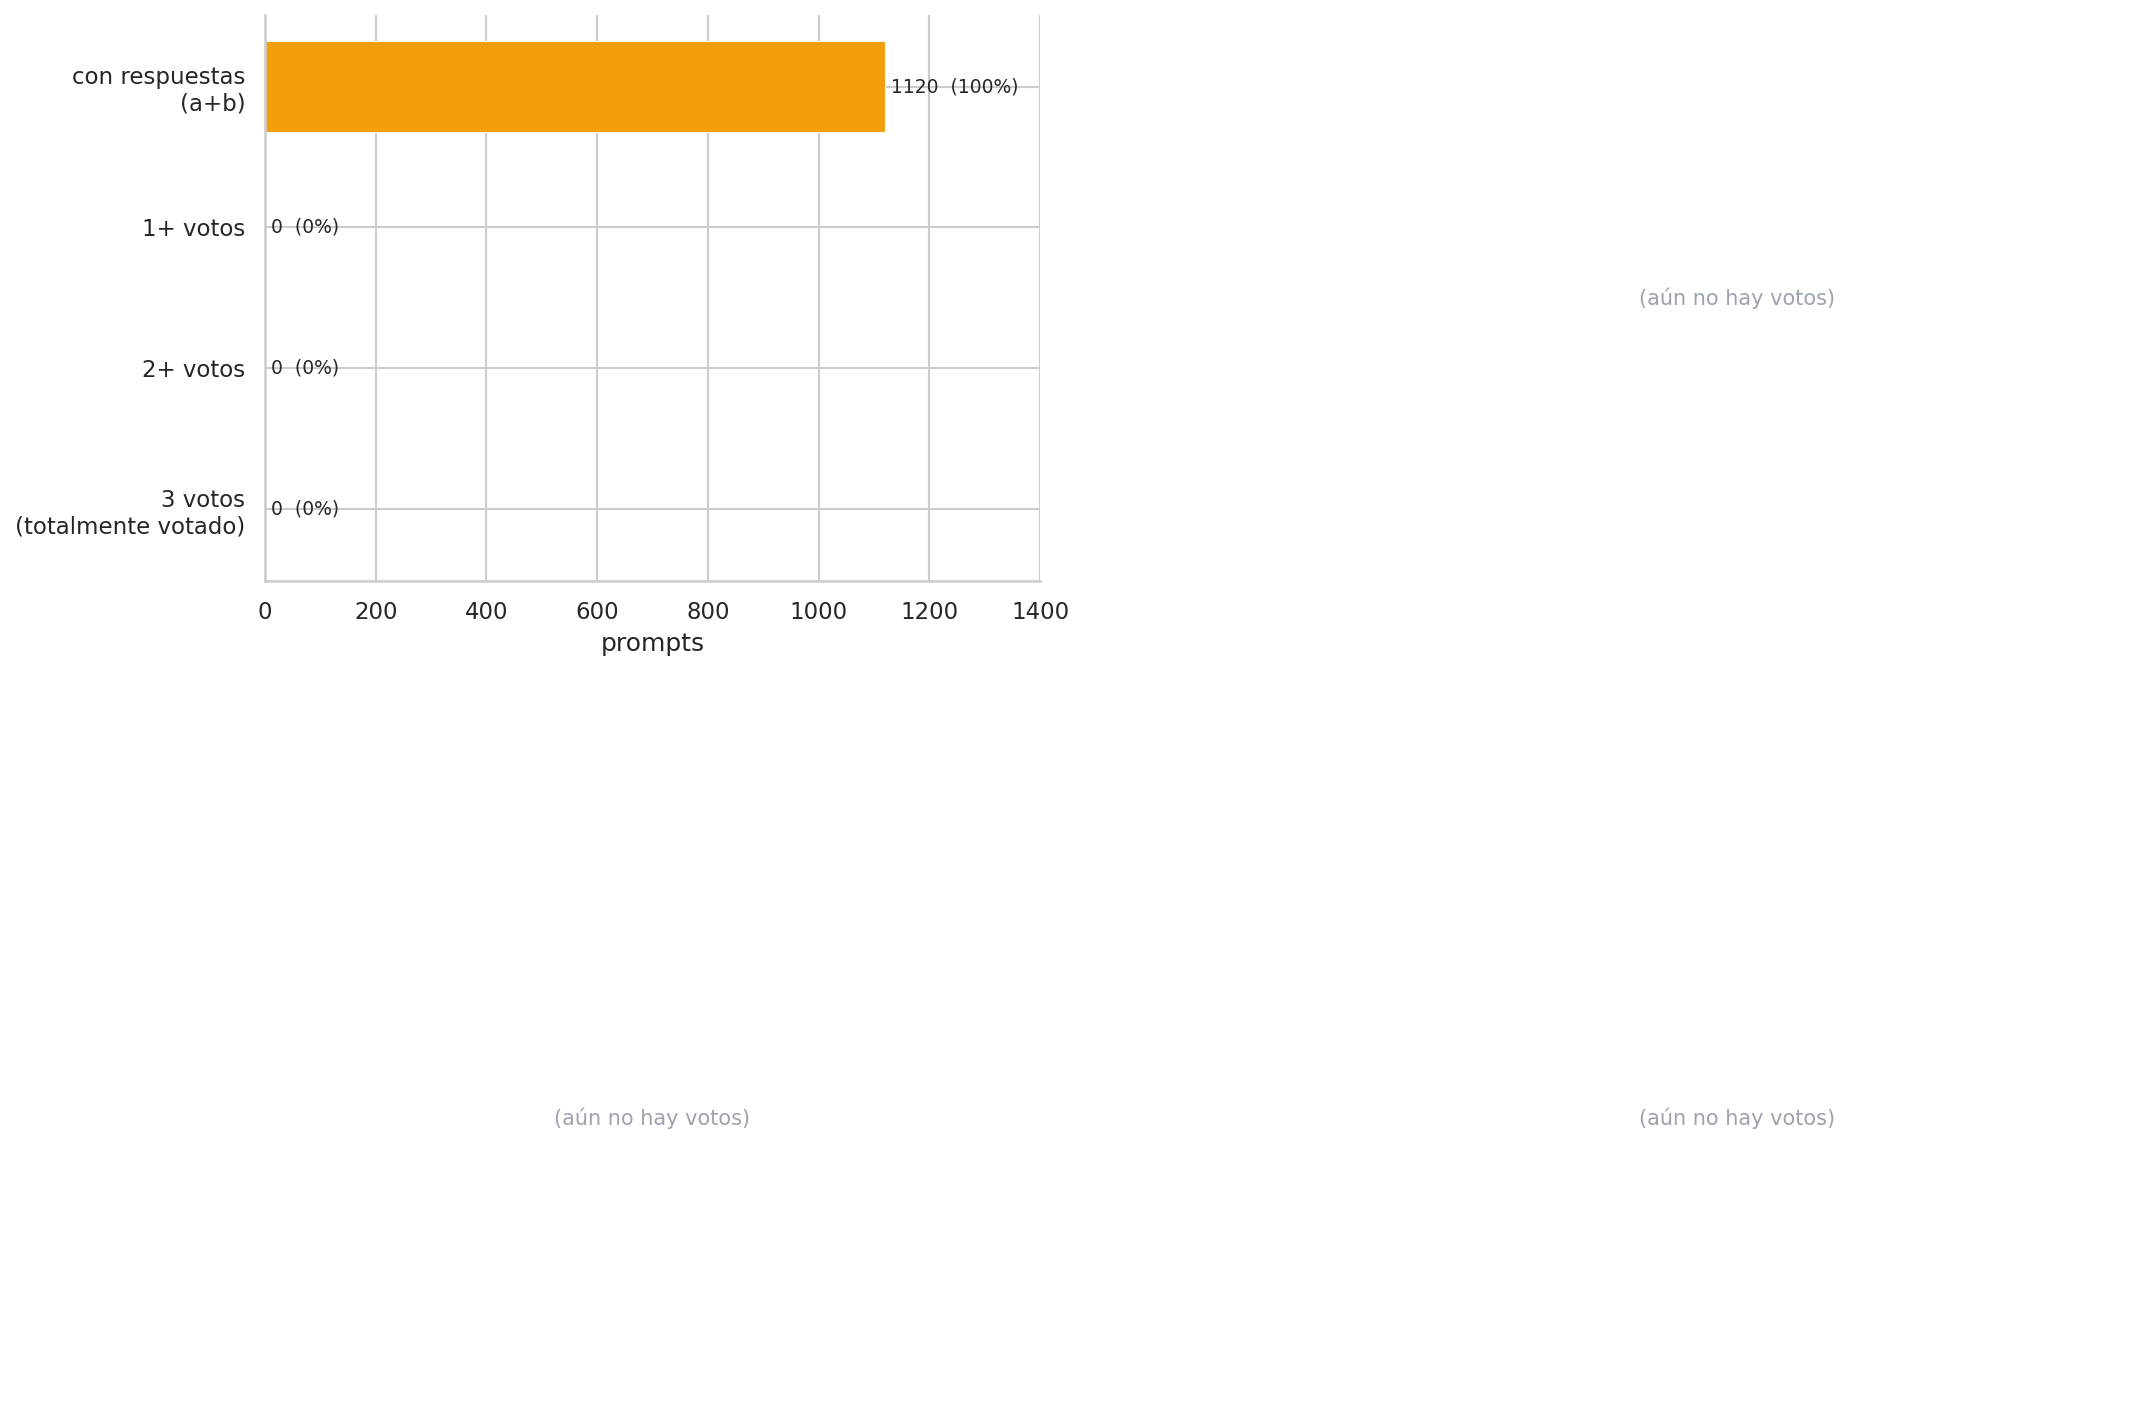
\includegraphics[width=0.95\textwidth]{panorama_votacion.png}
    \caption{Panorama de la votación de respuestas. Panel superior izquierdo: embudo del estado del pipeline de votación, empezando por los prompts con par $(a,b)$ de respuestas y avanzando a 1, 2 y 3 votos. Panel superior derecho: distribución de las elecciones del votante (A / B / ambas / ninguna). Panel inferior izquierdo: \textit{forest plot} con la tasa de victoria de cada modelo y su intervalo de confianza de Wilson al 95\%; la línea discontinua marca el 50\%. Panel inferior derecho: porcentaje de votos en los que el votante eligió 'ambas' o 'ninguna' cuando el modelo formaba parte del par — una alta tasa indica que el modelo tiende a quedar emparejado en comparaciones poco discriminantes.}
    \label{fig:panorama_votacion}
\end{figure}
